\documentclass{report}
\usepackage{tikz, calc}
\usepackage{comment}
\usepackage{xifthen}
\usepackage{amsmath}
\usepackage{lscape}

\usetikzlibrary{positioning}
\definecolor{myyellow}{RGB}{255,250,205}

\begin{document}

\begin{landscape} %horizontal page 
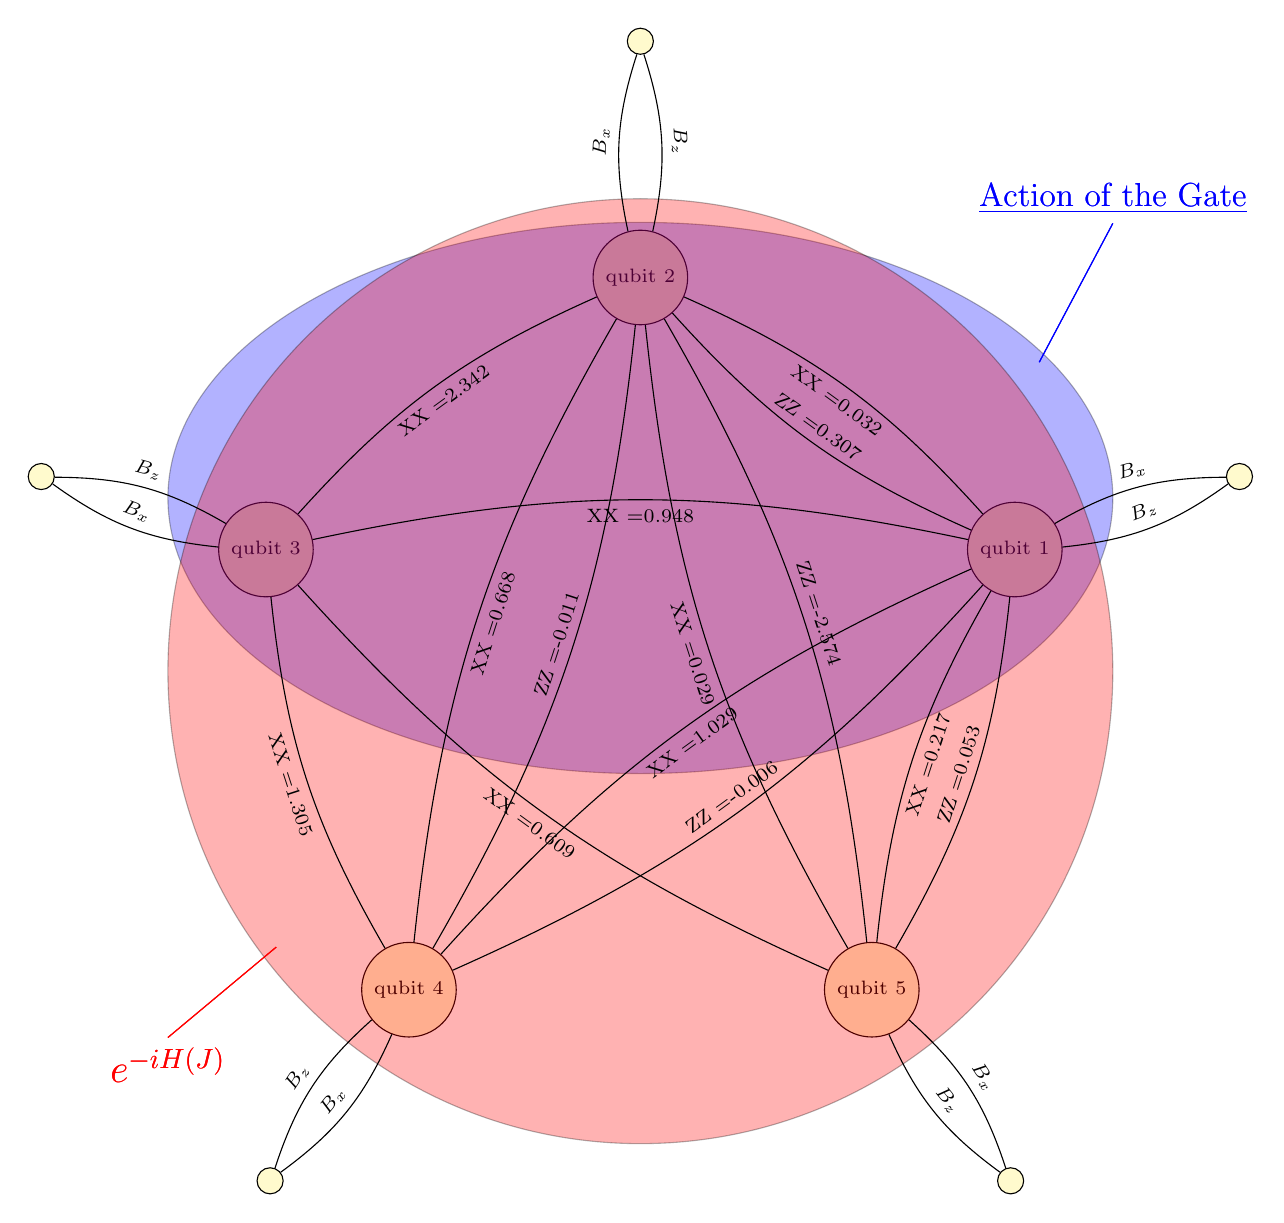
\begin{tikzpicture}



\foreach \a in {1,2,...,5}{
	\draw (\a*360/5 - 54: 5cm) node [circle, draw, fill = myyellow, align=center] (\a) {\scriptsize qubit \a};
};
\foreach \b in {6,...,10}{
	\draw (\b*360/5 - 54: 8cm) node [circle, draw, fill = myyellow, align=center] (\b) {};
};


\node [yshift = 6cm, xshift = 6cm] (no) {\large \color{blue} \underline {Action of the Gate}};
\node [yshift = 3.8cm, xshift = 5cm] (fi) {}
	edge[bend right=0, color= blue] (no.south);

\node [yshift = -5cm, xshift = -6cm] (no) {\Large \color{red} $e^{-i H ( J )}$};
\node [yshift = -3.4cm, xshift = -4.5cm] (fi) {}
	edge[bend right=0, color= red] (no.north);


%---------ELLIPSE-----------%
\draw [draw=black, fill=blue, opacity=0.3, align=left] (0,2.2) ellipse (6cm and 3.5cm);

\draw [draw=black, fill=red, opacity=0.3, align=left] (0,0) ellipse (6cm and 6cm);

%----------INNER LINKS-------------%

\draw[-]
(2) to [bend left = 12] node[sloped, below] {\scriptsize XX =0.032} (1);
\draw[-]
(2) to [bend right = 12] node[sloped, above] {\scriptsize ZZ =0.307} (1);
\draw[-]
(3) to [bend left = 12] node[sloped, below] {\scriptsize XX =0.948} (1);
\draw[-]
(3) to [bend left = 12] node[sloped, below] {\scriptsize XX =2.342} (2);
\draw[-]
(4) to [bend left = 12] node[sloped, below] {\scriptsize XX =1.029} (1);
\draw[-]
(4) to [bend right = 12] node[sloped, above] {\scriptsize ZZ =-0.006} (1);
\draw[-]
(4) to [bend left = 12] node[sloped, below] {\scriptsize XX =0.668} (2);
\draw[-]
(4) to [bend right = 12] node[sloped, above] {\scriptsize ZZ =-0.011} (2);
\draw[-]
(4) to [bend left = 12] node[sloped, below] {\scriptsize XX =1.305} (3);
\draw[-]
(5) to [bend left = 12] node[sloped, below] {\scriptsize XX =0.217} (1);
\draw[-]
(5) to [bend right = 12] node[sloped, above] {\scriptsize ZZ =0.053} (1);
\draw[-]
(5) to [bend left = 12] node[sloped, below] {\scriptsize XX =0.029} (2);
\draw[-]
(5) to [bend right = 12] node[sloped, above] {\scriptsize ZZ =-2.574} (2);
\draw[-]
(5) to [bend left = 12] node[sloped, below] {\scriptsize XX =0.609} (3);
%---------EXTERNAL LINKS-------%

\foreach \x/\y in {1/6,2/7,3/8,4/9,5/10}{

	\draw[-] 
	  (\x) to [bend right = -15] node[sloped, above] {\scriptsize $B_x$} (\y); 
	
	\draw[-] 
	  (\x) to [bend right = 15] node[sloped, above] {\scriptsize $B_z$} (\y); 
};


%--------COMMENTS-----------%

\node [yshift = 6cm, xshift = 6cm] (no) {\large \color{blue} \underline {Action of the Gate}};
\node [yshift = 3.8cm, xshift = 5cm] (fi) {}
	edge[bend right=0, color= blue] (no.south);

\node [yshift = -5cm, xshift = -6cm] (no) {\Large \color{red} $e^{-i H ( J )}$};
\node [yshift = -3.4cm, xshift = -4.5cm] (fi) {}
	edge[bend right=0, color= red] (no.north);


\end{tikzpicture}
\end{landscape}

\end{document}

